\section{tasks::sumflat Class Reference}
\label{classtasks_1_1sumflat}\index{tasks::sumflat@{tasks::sumflat}}
Inheritance diagram for tasks::sumflat::\begin{figure}[H]
\begin{center}
\leavevmode
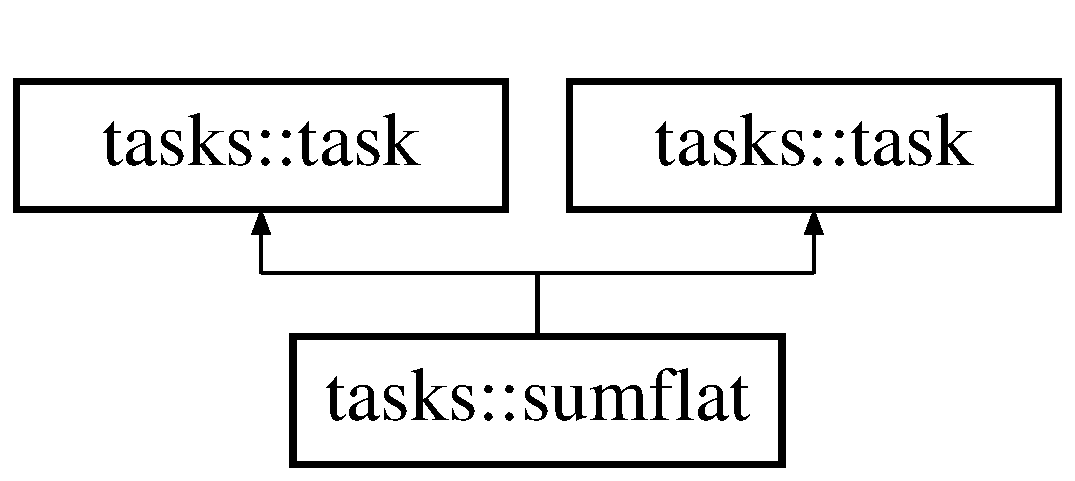
\includegraphics[height=2cm]{classtasks_1_1sumflat}
\end{center}
\end{figure}
\subsection*{Public Member Functions}
\begin{CompactItemize}
\item 
def \textbf{run}\label{classtasks_1_1sumflat_dcb4128b123f41178db6b333be3d7f2b}

\item 
def \textbf{run}\label{classtasks_1_1sumflat_dcb4128b123f41178db6b333be3d7f2b}

\end{CompactItemize}
\subsection*{Static Public Attributes}
\begin{CompactItemize}
\item 
string \textbf{name} = '{\bfsumflat}'\label{classtasks_1_1sumflat_bef7b115eafa9c85d54d98b6152616be}

\item 
string \textbf{button\-Text} = 'Create combined FLAT'\label{classtasks_1_1sumflat_07e6378f44986d26d46d9defba1325b7}

\end{CompactItemize}


\subsection{Detailed Description}


\footnotesize\begin{verbatim}Combine a set of FLAT frames into the combined FLAT frame. The
   currently implemented method is averaging of the images.
\end{verbatim}
\normalsize
 



The documentation for this class was generated from the following files:\begin{CompactItemize}
\item 
old/PANICtool-1.0/tasks.py\item 
old/tasks.py\end{CompactItemize}
